\documentclass{standalone}
\usepackage{tikz}
\usetikzlibrary{patterns, positioning}

\begin{document}
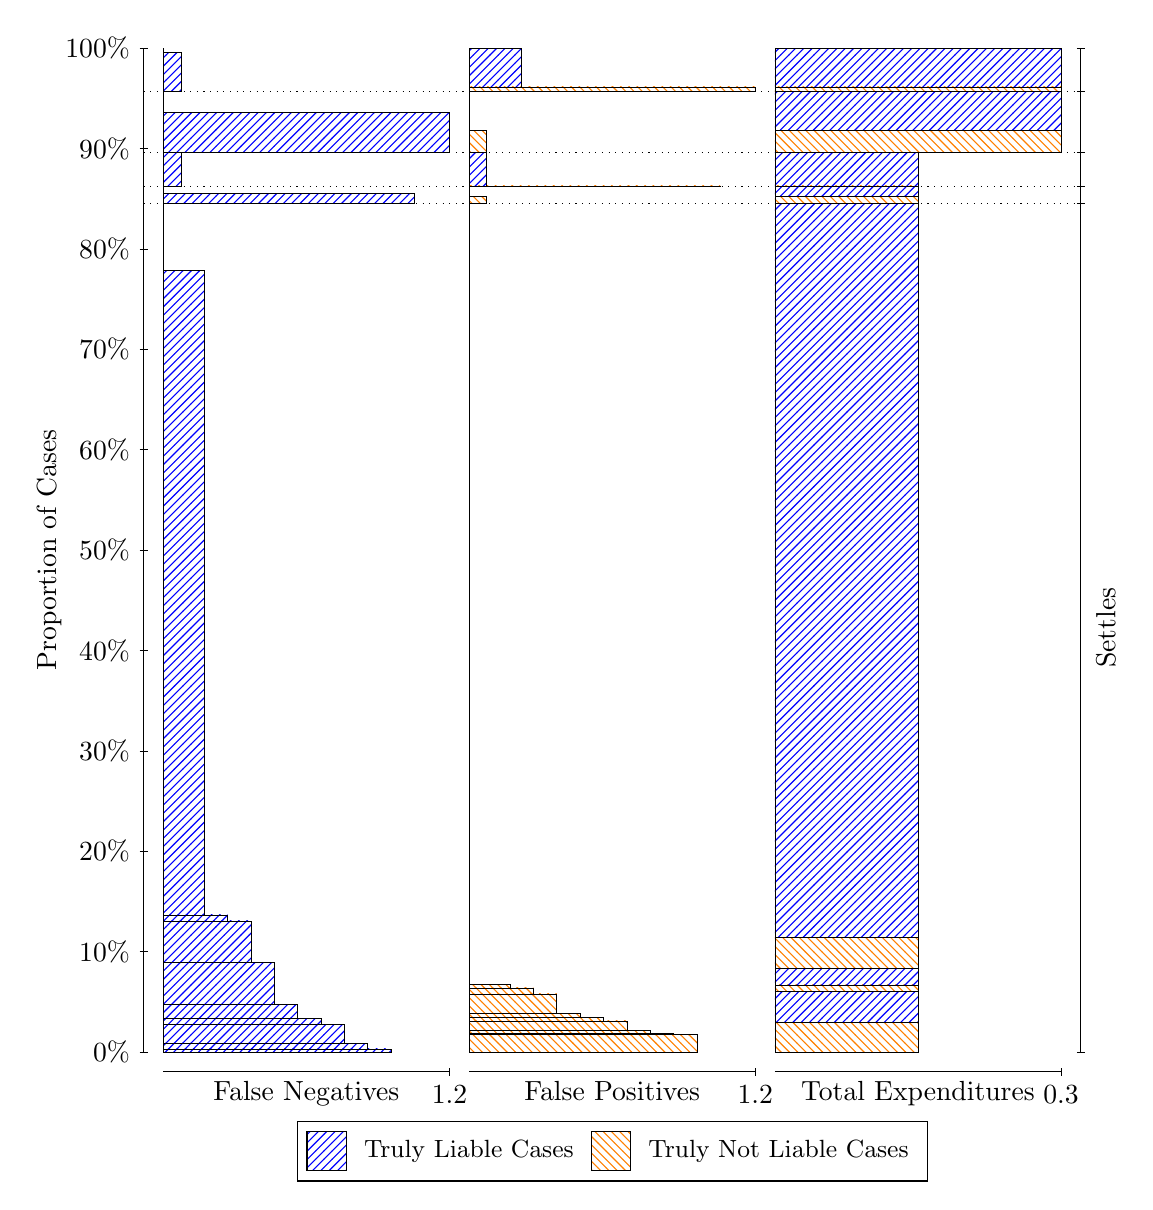
\begin{tikzpicture}
\draw[black, very thin] (1.5,1.75) -- (1.5,14.5);
\node[rotate=90, anchor=center] at (0.3, 8.125) {Proportion of Cases};
\draw[black, very thin] (1.45,1.75) -- (1.55,1.75);
\node[anchor=east] at (1.45, 1.75) {0\%};
\draw[black, very thin] (1.45,3.025) -- (1.55,3.025);
\node[anchor=east] at (1.45, 3.025) {10\%};
\draw[black, very thin] (1.45,4.3) -- (1.55,4.3);
\node[anchor=east] at (1.45, 4.3) {20\%};
\draw[black, very thin] (1.45,5.575) -- (1.55,5.575);
\node[anchor=east] at (1.45, 5.575) {30\%};
\draw[black, very thin] (1.45,6.85) -- (1.55,6.85);
\node[anchor=east] at (1.45, 6.85) {40\%};
\draw[black, very thin] (1.45,8.125) -- (1.55,8.125);
\node[anchor=east] at (1.45, 8.125) {50\%};
\draw[black, very thin] (1.45,9.4) -- (1.55,9.4);
\node[anchor=east] at (1.45, 9.4) {60\%};
\draw[black, very thin] (1.45,10.675) -- (1.55,10.675);
\node[anchor=east] at (1.45, 10.675) {70\%};
\draw[black, very thin] (1.45,11.95) -- (1.55,11.95);
\node[anchor=east] at (1.45, 11.95) {80\%};
\draw[black, very thin] (1.45,13.225) -- (1.55,13.225);
\node[anchor=east] at (1.45, 13.225) {90\%};
\draw[black, very thin] (1.45,14.5) -- (1.55,14.5);
\node[anchor=east] at (1.45, 14.5) {100\%};

\draw[black, very thin] (13.4,1.75) -- (13.4,14.5);
\draw[black, very thin] (13.35,1.75) -- (13.45,1.75);
\node[anchor=west] at (13.35, 1.75) {};
\draw[black, very thin] (13.35,12.527) -- (13.45,12.527);
\node[anchor=west] at (13.35, 12.527) {};
\draw[black, very thin] (13.35,12.743) -- (13.45,12.743);
\node[anchor=west] at (13.35, 12.743) {};
\draw[black, very thin] (13.35,13.178) -- (13.45,13.178);
\node[anchor=west] at (13.35, 13.178) {};
\draw[black, very thin] (13.35,13.951) -- (13.45,13.951);
\node[anchor=west] at (13.35, 13.951) {};
\draw[black, very thin] (13.35,14.5) -- (13.45,14.5);
\node[anchor=west] at (13.35, 14.5) {};

\draw[black, very thin, pattern color=blue, pattern=north east lines] (1.75,1.75) rectangle (4.6418,1.7895);
\draw[black, very thin, pattern color=blue, pattern=north east lines] (1.75,1.7895) rectangle (4.3452,1.855);
\draw[black, very thin, pattern color=blue, pattern=north east lines] (1.75,1.855) rectangle (4.0486,2.1009);
\draw[black, very thin, pattern color=blue, pattern=north east lines] (1.75,2.1009) rectangle (3.752,2.18);
\draw[black, very thin, pattern color=blue, pattern=north east lines] (1.75,2.18) rectangle (3.4554,2.3545);
\draw[black, very thin, pattern color=blue, pattern=north east lines] (1.75,2.3545) rectangle (3.1588,2.8891);
\draw[black, very thin, pattern color=blue, pattern=north east lines] (1.75,2.8891) rectangle (2.8622,3.4142);
\draw[black, very thin, pattern color=blue, pattern=north east lines] (1.75,3.4142) rectangle (2.5656,3.4905);
\draw[black, very thin, pattern color=blue, pattern=north east lines] (1.75,3.4905) rectangle (2.269,11.673);
\draw[black, very thin, pattern color=orange, pattern=north west lines] (1.75,11.673) rectangle (1.75,12.527);
\draw[black, very thin, pattern color=blue, pattern=north east lines] (1.75,12.527) rectangle (4.9384,12.654);
\draw[black, very thin, pattern color=orange, pattern=north west lines] (1.75,12.654) rectangle (1.75,12.743);
\draw[black, very thin, pattern color=blue, pattern=north east lines] (1.75,12.743) rectangle (1.9724,13.173);
\draw[black, very thin, pattern color=orange, pattern=north west lines] (1.75,13.173) rectangle (1.75,13.178);
\draw[black, very thin, pattern color=blue, pattern=north east lines] (1.75,13.178) rectangle (5.3833,13.679);
\draw[black, very thin, pattern color=orange, pattern=north west lines] (1.75,13.679) rectangle (1.75,13.951);
\draw[black, very thin, pattern color=blue, pattern=north east lines] (1.75,13.951) rectangle (1.9724,14.445);
\draw[black, very thin, pattern color=orange, pattern=north west lines] (1.75,14.445) rectangle (1.75,14.5);
\draw[black, very thin, pattern color=orange, pattern=north west lines] (5.6333,1.75) rectangle (8.5252,1.9769);
\draw[black, very thin, pattern color=orange, pattern=north west lines] (5.6333,1.9769) rectangle (8.2286,1.9884);
\draw[black, very thin, pattern color=orange, pattern=north west lines] (5.6333,1.9884) rectangle (7.932,2.0284);
\draw[black, very thin, pattern color=orange, pattern=north west lines] (5.6333,2.0284) rectangle (7.6354,2.1443);
\draw[black, very thin, pattern color=orange, pattern=north west lines] (5.6333,2.1443) rectangle (7.3388,2.1883);
\draw[black, very thin, pattern color=orange, pattern=north west lines] (5.6333,2.1883) rectangle (7.0422,2.2426);
\draw[black, very thin, pattern color=orange, pattern=north west lines] (5.6333,2.2426) rectangle (7.0422,2.2426);
\draw[black, very thin, pattern color=orange, pattern=north west lines] (5.6333,2.2426) rectangle (6.7456,2.4881);
\draw[black, very thin, pattern color=orange, pattern=north west lines] (5.6333,2.4881) rectangle (6.449,2.5631);
\draw[black, very thin, pattern color=orange, pattern=north west lines] (5.6333,2.5631) rectangle (6.1524,2.6046);
\draw[black, very thin, pattern color=blue, pattern=north east lines] (5.6333,2.6046) rectangle (5.6333,12.527);
\draw[black, very thin, pattern color=orange, pattern=north west lines] (5.6333,12.527) rectangle (5.8558,12.616);
\draw[black, very thin, pattern color=blue, pattern=north east lines] (5.6333,12.616) rectangle (5.6333,12.743);
\draw[black, very thin, pattern color=orange, pattern=north west lines] (5.6333,12.743) rectangle (8.8218,12.748);
\draw[black, very thin, pattern color=blue, pattern=north east lines] (5.6333,12.748) rectangle (5.8558,13.178);
\draw[black, very thin, pattern color=orange, pattern=north west lines] (5.6333,13.178) rectangle (5.8558,13.45);
\draw[black, very thin, pattern color=blue, pattern=north east lines] (5.6333,13.45) rectangle (5.6333,13.951);
\draw[black, very thin, pattern color=orange, pattern=north west lines] (5.6333,13.951) rectangle (9.2667,14.006);
\draw[black, very thin, pattern color=blue, pattern=north east lines] (5.6333,14.006) rectangle (6.3007,14.5);
\draw[black, very thin, pattern color=orange, pattern=north west lines] (9.5167,1.75) rectangle (11.333,2.1249);
\draw[black, very thin, pattern color=blue, pattern=north east lines] (9.5167,2.1249) rectangle (11.333,2.5153);
\draw[black, very thin, pattern color=orange, pattern=north west lines] (9.5167,2.5153) rectangle (11.333,2.6007);
\draw[black, very thin, pattern color=blue, pattern=north east lines] (9.5167,2.6007) rectangle (11.333,2.8148);
\draw[black, very thin, pattern color=orange, pattern=north west lines] (9.5167,2.8148) rectangle (11.333,3.2091);
\draw[black, very thin, pattern color=blue, pattern=north east lines] (9.5167,3.2091) rectangle (11.333,12.527);
\draw[black, very thin, pattern color=orange, pattern=north west lines] (9.5167,12.527) rectangle (11.333,12.616);
\draw[black, very thin, pattern color=blue, pattern=north east lines] (9.5167,12.616) rectangle (11.333,12.743);
\draw[black, very thin, pattern color=orange, pattern=north west lines] (9.5167,12.743) rectangle (11.333,12.748);
\draw[black, very thin, pattern color=blue, pattern=north east lines] (9.5167,12.748) rectangle (11.333,13.178);
\draw[black, very thin, pattern color=orange, pattern=north west lines] (9.5167,13.178) rectangle (13.15,13.45);
\draw[black, very thin, pattern color=blue, pattern=north east lines] (9.5167,13.45) rectangle (13.15,13.951);
\draw[black, very thin, pattern color=orange, pattern=north west lines] (9.5167,13.951) rectangle (13.15,14.006);
\draw[black, very thin, pattern color=blue, pattern=north east lines] (9.5167,14.006) rectangle (13.15,14.5);
\draw[black, dotted] (1.5,12.527) -- (13.4,12.527);
\draw[black, dotted] (1.5,12.743) -- (13.4,12.743);
\draw[black, dotted] (1.5,13.178) -- (13.4,13.178);
\draw[black, dotted] (1.5,13.951) -- (13.4,13.951);
\draw[black, very thin] (1.75,1.5) -- (5.3833,1.5);
\node[anchor=north] at (3.5667, 1.5) {False Negatives};
\draw[black, very thin] (5.3833,1.45) -- (5.3833,1.55);
\node[anchor=north] at (5.3833, 1.45) {1.2};

\draw[black, very thin] (5.6333,1.5) -- (9.2667,1.5);
\node[anchor=north] at (7.45, 1.5) {False Positives};
\draw[black, very thin] (9.2667,1.45) -- (9.2667,1.55);
\node[anchor=north] at (9.2667, 1.45) {1.2};

\draw[black, very thin] (9.5167,1.5) -- (13.15,1.5);
\node[anchor=north] at (11.333, 1.5) {Total Expenditures};
\draw[black, very thin] (13.15,1.45) -- (13.15,1.55);
\node[anchor=north] at (13.15, 1.45) {0.3};

\node[black, centered, rotate=90] at (13.72, 7.1386) {Settles};





\draw (7.449999999999999,1.5) node[draw=none] (baseCoordinate) {};
\begin{scope}[align=center]
        \matrix[scale=0.5, draw=black, below=0.5cm of baseCoordinate, nodes={draw}, column sep=0.1cm]{
            \node[rectangle, draw, minimum width=0.5cm, minimum height=0.5cm, pattern=north east lines, pattern color=blue] {}; &
            \node[draw=none, font=\small] (B) {Truly Liable Cases}; &
            \node[rectangle, draw, minimum width=0.5cm, minimum height=0.5cm, pattern=north west lines, pattern color=orange] {}; &
            \node[draw=none, font=\small] (B) {Truly Not Liable Cases}; \\
            };
\end{scope}

\end{tikzpicture}
\end{document}